%%%%%%%%%%%%%%%%%%%%%%%%%%%%%%%%%%%%%%%%%%%%%%%%%%%%%%%%%%%%
% METHODS
%%%%%%%%%%%%%%%%%%%%%%%%%%%%%%%%%%%%%%%%%%%%%%%%%%%%%%%%%%%%
\section{Methods}\label{sec:methods}

\subsection{Overview}

To solve physics-informed forward and inverse problems under uncertainty, we start by pre-training a diffusion generative model on a family of partial differential equations (PDEs). This model is designed to learn the joint distribution of the PDE coefficients (or the initial state) and its corresponding solutions (or the final state). Our approach involves recovering full data in both spaces using sparse observations from either or both sides. We achieve this through the iterative denoising of random Gaussian noise as in regular diffusion models but with additional guidance from the sparse observations and the PDE function enforced during denoising. The schematic description of our approach is shown in Fig. \ref{fig:architecture}.

\subsection{Prelimary: Diffusion Models and Guided Diffusion}

Diffusion models involve a predefined forward process that gradually adds Gaussian noise to the data and a learned reverse process that denoises the data to reconstruct the original distribution. Specifically, Song et al. \cite{song2021scorebased} propose a deterministic diffusion model that learns an $N$-step denoising process that eventually outputs a denoised data $\x_N$ and satisfies the following ordinary differential equations (ODE) at each timestep $t_i$ where $i\in \{0,1,...,N-1\}$
\begin{equation}
    \label{eq:ode}
    \mathrm{d}\x=-\dot{\sigma}(t) \sigma(t) \nabla_{\x}\log p\big(\x;\sigma(t)\big) \mathrm{d}t.
\end{equation}
Here $\nabla_{\x}\log p\big(\x;\sigma(t)\big)$  is the score function \cite{hyvarinen2005estimation} that helps to transform samples from a normal distribution $\N(0,\sigma(t_0)^2\I)$ to a target probability distribution $p(\x;\sigma(t))$. To estimate the score function, Karras et al. \cite{Karras2022edm} propose to learn a denoiser function $D(\x;\sigma)$ such that
\begin{equation}
    \nabla_{\x}\log p\big(\x;\sigma(t)\big)=(D(\x;\sigma(t))-\x)/\sigma(t)^2
\end{equation}

To enable control over the generated data, guided diffusion methods \cite{dhariwal2021diffusion} add guidance gradients to the score function during the denoising process. Recently, diffusion posterior sampling (DPS) \cite{chung2022diffusion} made notable progress in guided diffusion for tackling various inverse problems. DPS uses corrupted measurements $\y$ derived from $\x$ to guide the diffusion model in outputting the posterior distribution $p(\x|\y)$. A prime application of DPS is the inpainting problem, which involves recovering a complete image from sparsely observed pixels, which suits well with our task. This approach modifies Eq. \ref{eq:ode} to
\begin{equation}
    \label{eq:ode-dps}
    \mathrm{d}\x = -\dot{\sigma}(t) \sigma(t) \big(\nabla_{\x}\log p\big(\x;\sigma(t)\big)+\nabla_{\x}\log p\big(\y|\x;\sigma(t)\big)\big)\mathrm{d}t.
\end{equation}

DPS \cite{chung2022diffusion} showed that under Gaussian noise assumption of the sparse measurement operator $\mathcal{M}(\cdot)$, i.e., $\y|\x \sim \mathcal{N}(\mathcal{M}(\x), \delta^2\I)$ with some S.D. $\delta$, the log-likelihood function can be approximated with:
\begin{equation}
    \nabla_{\x}\log p\big(\y|\x_i;\sigma(t_i)\big)\approx \nabla_{\x_i}\log p\big(\y|\hatx_N^i;\sigma(t_i)\big)\approx -\frac1{\delta^2}\nabla_{\x_i}\|\y-\mathcal{M}(\hat{\x}_N^i(\x_i;\sigma(t_i))\|_2^2,
\end{equation}
where $\hat{\x}_N^i:=D(\x_i;\sigma(t_i))$ denotes the estimation of the final denoised data at each denoising step $i$. Applying the Baye's rule, the gradient direction of the guided diffusion is therefore:
\begin{equation}\label{eq:dps-posterior}
    \nabla_{\x_i}\log p(\x_i|\y)\approx s(\x_i)-\zeta\nabla_{\x_i}\|\y-\mathcal{M}(\hat{\x}_N^i)\|_2^2,
\end{equation}
where $s(\x)=\nabla_{\x}\log p\big(\x\big)$ is the original score function, and $\zeta=1/\delta^2$. 

\begin{algorithm}[!tbp]
	\caption{Sparse Observation and PDE Guided Diffusion Sampling Algorithm.}
	\label{alg1}
	\begin{algorithmic}[1]
		\State \textbf{input} DeterministicSampler $D_\theta(\textit{\textbf{x}};\sigma), ~\sigma(t_{i \in \{0, \dots, N\}})$, TotalPointCount $m$, ObservedPointCount $n$, Observation $\y$, PDEFunction $f$, Weights $\zeta_{obs}, \zeta_{pde}$
            \State \textbf{sample} $\textit{\textbf{x}}_0 \sim \N \big( \mathbf{0}, ~\sigma(t_0)^2\mathbf{I}\big)$\mycomment Generate initial sampling noise
            \For{$i \in \{0, \dots, N-1\}$}
                \State $\hatx_N^i\leftarrow D_{\theta}\left(\x_{i} ; \sigma(t_{i})\right)$\mycomment Estimate the denoised data at step $t_{i}$
                \State $\boldsymbol{d}_{i} \leftarrow\left(\x_{i}-\hatx_N^i\right) / \sigma(t_{i})$\mycomment Evaluate $\mathrm{d}\boldsymbol{x}/\mathrm{d}\sigma(t)$ at step $t_i$
                \State $\x_{i+1}\leftarrow \x_{i}+(\sigma(t_{i+1})-\sigma(t_i))\boldsymbol{d}_{i}$\mycomment Take an Euler step from $\sigma(t_i)$ to $\sigma(t_{i+1})$
                \If{$\sigma(t_{i+1})\neq 0$}
                    \State $\hatx_N^i\leftarrow D_\theta(\x_{i+1};\sigma(t_{i+1}))$\mycomment Apply $2^{\mathrm{nd}}$ order correlation unless $\sigma=0$
                    \State $\boldsymbol{d}_i^{\prime}\leftarrow\left(\x_{i+1}-\hatx_N^i\right)/\sigma(t_{i+1})$\mycomment Evaluate $\mathrm{d}\boldsymbol{x}/\mathrm{d}\sigma(t)$ at step $t_{i+1}$
                    \State $\x_{i+1}\leftarrow\x_i+(\sigma(t_{i+1})-\sigma(t_i))\left(\frac12\boldsymbol{d}_i+\frac12\boldsymbol{d}_i^{\prime}\right)$\mycomment Apply the trapezoidal rule at step $t_{i+1}$
                \EndIf
                \State $\mathcal{L}_{obs} \leftarrow \frac1n\|\y-\hat{\x}_N^i\|_2^2$ \mycomment Evaluate the observation loss of $\hatx_N^i$
                \State $\mathcal{L}_{pde} \leftarrow \frac1m\|\mathbf{0}-f(\hat{\x}_N^i)\|_2^2$ \mycomment Evaluate the PDE loss of $\hatx_N^i$
                \State $\x_{i+1} \leftarrow \x_{i+1} - \zeta_{obs}\nabla_{\x_i}\mathcal{L}_{obs} - \zeta_{pde}\nabla_{\x_i}\mathcal{L}_{pde}$ \mycomment Guide the sampling with $\mathcal{L}_{obs}$ and $\mathcal{L}_{pde}$
            \EndFor
            \State \textbf{return} $\x_N$ \mycomment Return the denoised data
    \end{algorithmic}  
\end{algorithm}

\subsection{Solving PDEs with Guided Diffusion}\label{sec:method}

Our work focuses on two classes of PDEs: static PDEs and dynamic time-dependent PDEs. Static systems (e.g., Darcy Flow or Poisson equations) are defined by a time-independent function $f$:
\begin{equation}\label{eq:static}
    \begin{aligned}
        f(\c;\a,\u)=0~\text{ in }~\Omega\subset\R^d, \quad\quad 
        \u(\c)=\boldsymbol{g}(\c)~\text{ in }~\partial \Omega,
    \end{aligned}
\end{equation}
where $\Omega$ is a bounded domain, $\c\in\Omega$ is a spatial coordinate, $\a\in\mathcal{A}$ is the PDE coefficient field, and $\u\in\mathcal{U}$ is the solution field. $\partial \Omega$ is the boundary of the domain $\Omega$ and $\u|_{\partial\Omega} = \boldsymbol{g}$ is the boundary constraint. We aim to recover both $\a$ and $\u$ from sparse observations on either $\a$ or $\u$ or both. 

Similarly, we consider the dynamic systems (e.g., Navier-Stokes):
\begin{equation}\label{eq:dynamic}
\begin{aligned}
% \begin{split}
    f(\c,\t;\a,\u)&=0, \quad&\text{in } \Omega \times (0,\infty) \\
    \u(\c,\t) &= \boldsymbol{g}(\c,\t), \quad&\text{in } \partial \Omega \times (0,\infty) \\
    \u(\c,\t) &= \a(\c,\t), \quad&\text{in } \bar{\Omega} \times \{0\}
% \end{split}
\end{aligned}
\end{equation}

where $\t$ is a temporal coordinate, $\a=\u_0\in\mathcal{A}$ is the initial condition, $\u$ is the solution field, and $\u|_{\Omega\times(0,\infty)} = \boldsymbol{g}$ is the boundary constraint. We aim to simultaneously recover both $\a$ and the solution $\u_T := \u(\cdot, T)$ at a specific time $T$ from sparse observations on either $\a$, $\u_T$, or both.  



Finally, we explore the recovery of the states across all timesteps $\u_{0:T}$ in 1D dynamic systems governed by Burger's equation. Our network $D_\theta$ models the distribution of all 1D states, including the initial condition $\u_0$ and solutions $\u_{1:T}$ stacked in the temporal dimension, forming a 2D dataset.

\paragraph{Guided Diffusion Algorithm}
In the data-driven PDE literature, the above tasks can be achieved by learning directional mappings between $\a$ and $\u$ (or $u_T$ for dynamic systems). Thus, existing methods typically train separate neural networks for the forward solution operator $\mathcal{F}:\mathcal{A}\rightarrow \mathcal{U}$ and the inverse solution operator $\mathcal{I}:\mathcal{U}\rightarrow \mathcal{A}$.


Our method unifies the forward and inverse operators with a single network and an algorithm using the guided diffusion framework. DiffusionPDE can handle arbitrary sparsity patterns with one pre-trained diffusion model $D_\theta$ that learns the joint distribution of $\mathcal{A}$ and $\mathcal{U}$, concatenated on the channel dimension, denoted $\mathcal{X}$. Thus, our data $\x \in \mathcal{X},$ where $\mathcal{X}:=\mathcal{A}\times \mathcal{U}.$ We follow the typical diffusion model procedures \cite{Karras2022edm} to train our model on a family of PDEs.


Once we train the diffusion model $D_\theta$, we employ our physics-informed DPS \cite{chung2022diffusion} formulation during inference to guide the sampling of $\x\in \mathcal{X}$ that satisfies the sparse observations and the given PDE, as detailed in Algorithm \ref{alg1}. We follow Eq.~\ref{eq:dps-posterior} to modify the score function using the two guidance terms:
\begin{equation}\label{eq:diffusionpde-loss}
    \nabla_{\x_i}\log p(\x_i|\y_{obs},f)\approx \nabla_{\x_i}\log p\big(\x_i)-\zeta_{obs}\nabla_{\x_i}\mathcal{L}_{obs}-\zeta_{pde}\nabla_{\x_i}\mathcal{L}_{pde},
\end{equation}
where $\x_i$ is the noisy data at denoising step $i$, $\y_{obs}$ are the observed values, and $f(\cdot)=\mathbf{0}$ is the underlying PDE condition. $\mathcal{L}_{obs}$ and $\mathcal{L}_{pde}$ respectively represent the MSE loss of the sparse observations and the PDE equation residuals:
\begin{equation}
    \begin{aligned}\label{eq:loss_terms}
    % \mathcal{L} &= \mathcal{L}_{obs} + \alpha \mathcal{L}_{pde}\\
    \mathcal{L}_{obs}(\x_i,\y_{obs};D_\theta) &=\frac{1}{n}\|\y_{obs}-\hat{\x}_N^i\|_2^2= \frac1n\sum_{j=1}^n(\y_{obs}(\o_j)-\hat{\x}_N^i(\o_j))^2, \\
\mathcal{L}_{pde}(\x_i;D_\theta,f)&=\frac{1}{m}\|\mathbf{0}-f(\hat{\x}_N^i)\|_2^2=\frac1m\sum_{j}\sum_k f(\c_j,\t_k;\hat{\u}_j,\hat{\a}_j)^2,
    \end{aligned}
\end{equation}
where $\hat{\x}_N^i=D_\theta(\x_i)$ is the clean image estimate at denoising timestep $i$, which can be split into coefficient $\hat{\u}_i$ and solution $\hat{\boldsymbol{a}}_i.$
Here, $m$ is the total number of grid points (i.e., pixels), $n$ is the number of sparse observation points. $\o_j$ represents the spatio-temporal coordinate of $j$th observation. Note that, without loss of generality, $\mathcal{L}_{pde}$ can be accumulated for all applicable PDE function $f$ in the system, and the time component $\t_k$ is ignored for static systems.

\begin{figure}[t!]
    \centering
    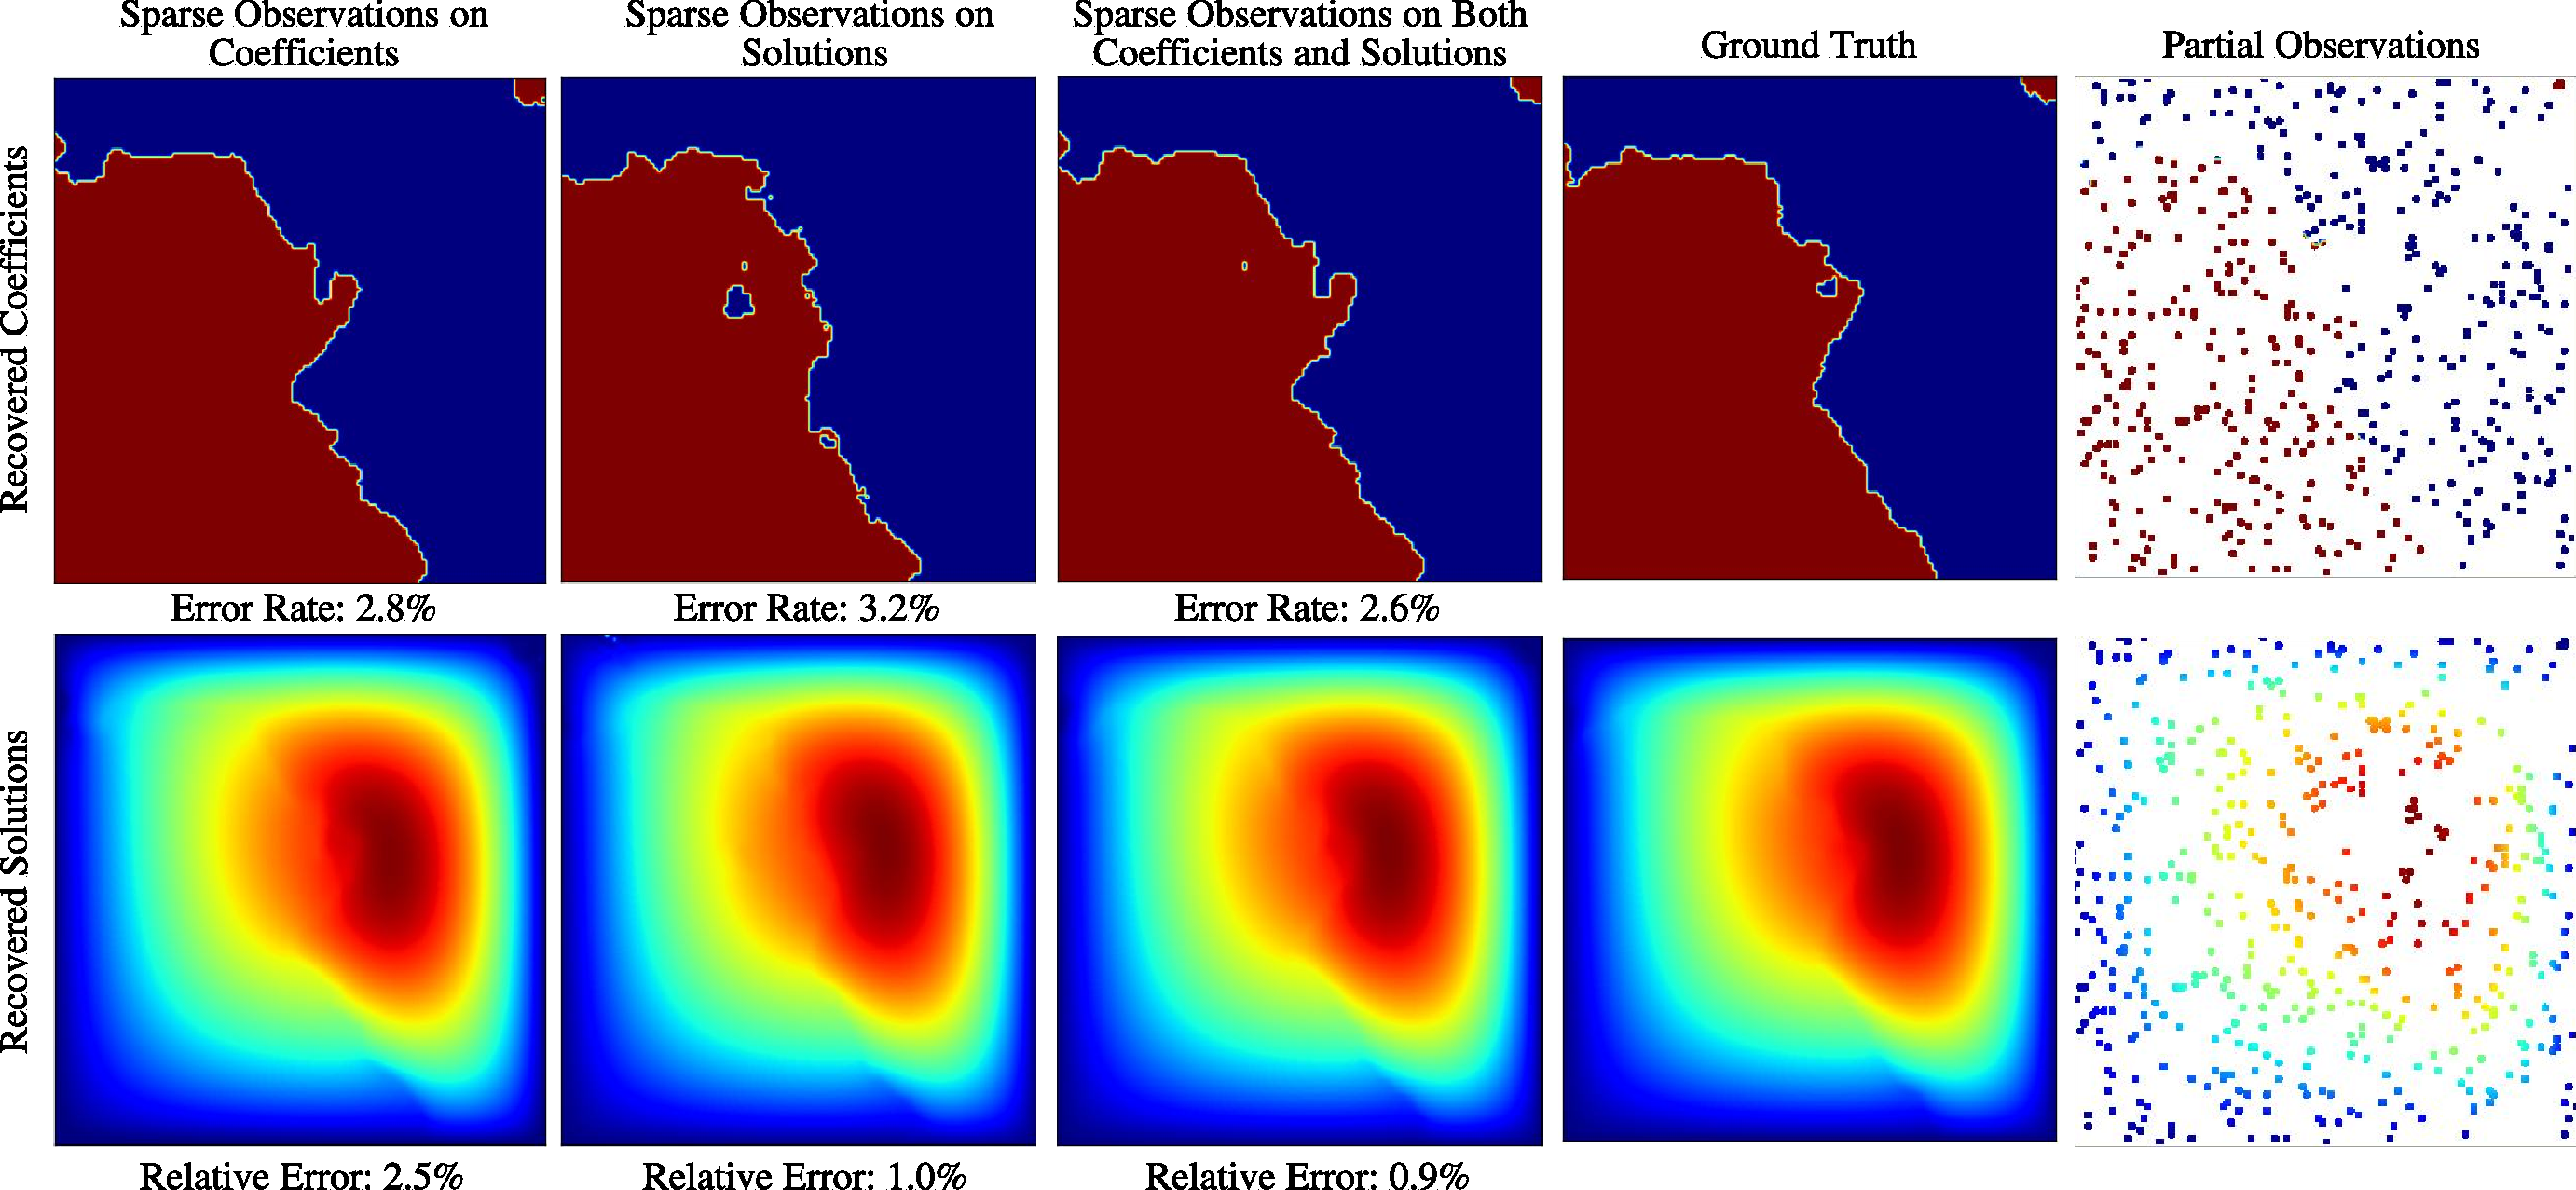
\includegraphics[width=0.85\textwidth]{figs/darcy/darcy_500a_u_au.pdf}
    \caption{Different from forward and inverse PDE solvers, DiffusionPDE can take sparse observations on either the coefficient $\a$ or the solution $\u$ to recover both of them, using one trained network. Here, we show the recovered $\a$ and $\u$ of the Darcy's eqaution given sparse observations on $\a$, $\u$, or both. Compared with the ground truth, we see that our method successfully recovers the PDE in all cases.}
    \label{fig:darcy_a_u_au}
\end{figure}

\begin{figure}[t!]
    \centering
    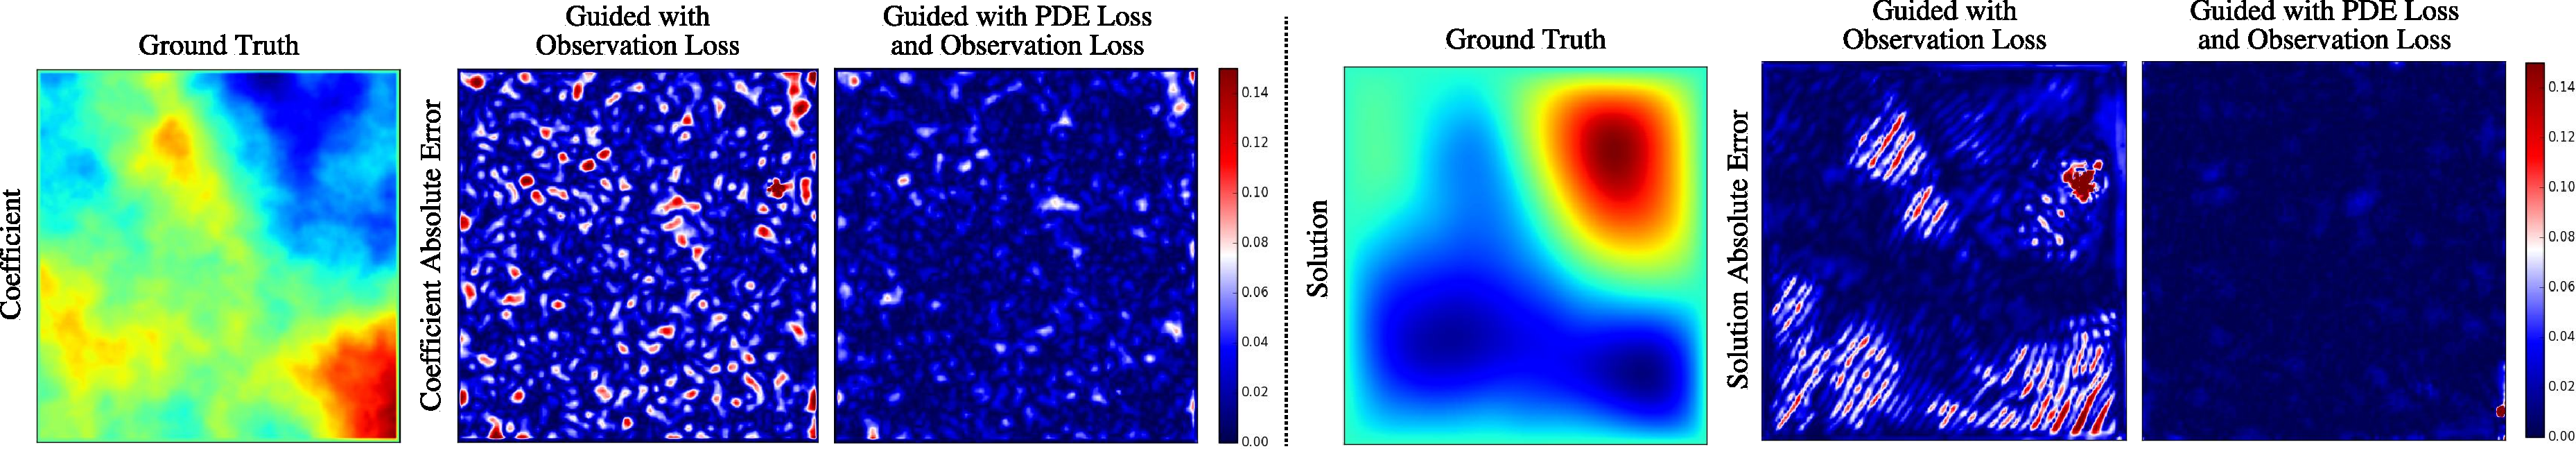
\includegraphics[width=0.99\textwidth]{figs/helmholtz/helmholtz_loss.pdf}
    \caption{Usefulness of PDE loss. We visualize the absolute errors of the recovered coefficient and solution of the Helmholtz equation with and w/o PDE loss. We compare having only the observation loss with applying the additional PDE loss. The errors drop significantly when using PDE loss.}
    \label{fig:helmholtz_pde}
\end{figure}
